\documentclass[a4paper,11pt]{article}

\usepackage{geometry}
\usepackage{listings}
\usepackage{mathrsfs}
\usepackage[font={small},labelfont={sf,bf}]{caption}
\usepackage{color}
\usepackage{amssymb}
\usepackage[utf8]{inputenc}
\usepackage{afterpage}
\usepackage[T1]{fontenc}
\usepackage{amsfonts}
\usepackage{mathtools}
\usepackage{amsmath}
\usepackage{verbatim}
\usepackage{bm}
\usepackage{bbm}
\usepackage{enumerate}
\usepackage{amsthm}
\usepackage{stmaryrd}

\geometry{a4paper,top=3cm,bottom=3cm,left=2cm,right=2cm,heightrounded, bindingoffset=5mm}

\theoremstyle{definition}
\newtheorem{definition}{Definition}[section]
\theoremstyle{plain}
\newtheorem{theo}[definition]{Theorem}
\newtheorem{prop}[definition]{Proposition}
\newtheorem{lemma}[definition]{Lemma}
\newtheorem{cor}[definition]{Corollary}
\newtheorem{ex}[definition]{Example}
\theoremstyle{remark}
\newtheorem{rem}[definition]{Remark}
\newtheorem{rem*}[definition]{}

\newcommand*\mcup{\mathbin{\mathpalette\mcupinn\relax}}
\newcommand*\mcupinn[2]{\vcenter{\hbox{$\mathsurround=0pt
  \ifx\displaystyle#1\textstyle\else#1\fi\bigcup$}}}
\newcommand*\mcap{\mathbin{\mathpalette\mcapinn\relax}}
\newcommand*\mcapinn[2]{\vcenter{\hbox{$\mathsurround=0pt
  \ifx\displaystyle#1\textstyle\else#1\fi\bigcap$}}}
\DeclarePairedDelimiter{\abs}{\lvert}{\rvert}
\DeclarePairedDelimiter{\norm}{\lVert}{\rVert}
\DeclarePairedDelimiter{\parr}{(}{)}
\DeclarePairedDelimiter{\parq}{[}{]}
\DeclarePairedDelimiter{\parqq}{\llbracket}{\rrbracket}
\DeclarePairedDelimiter{\bra}{\lbrace}{\rbrace}
\DeclarePairedDelimiter{\ceil}{\lceil}{\rceil}
\DeclarePairedDelimiter{\prodscal}{\langle}{\rangle}
\DeclarePairedDelimiter{\floor}{\lfloor}{\rfloor}
\DeclareMathOperator*{\argmin}{arg\,min}
\DeclareMathOperator*{\argmax}{arg\,max}
\DeclareMathOperator*{\expval}{\mathbb{E}}
\DeclareMathOperator*{\varval}{\mathrm{Var}}
\DeclareMathOperator*{\covval}{\mathrm{Cov}}

\begin{document}

\title{Applied Stochastic Analysis \\ Homework assignment 10}
\author{Luca Venturi}
\maketitle

\section*{Exercise 1}

\paragraph*{(a)}

By applying It\^o formula, we have
\begin{align*}
I^{(3)}_t & \doteq \int_0^t\int_0^{s_1}\int_0^{s_2} dW_{s_3}\,dW_{s_2}\,dW_{s_1} = \int_0^t\int_0^{s_1}W_{s_2}\,dW_{s_2}\,dW_{s_1} \\
& = \int_0^t\parq*{\int_0^{s_1}\,d\parr*{\frac{1}{2}W_{s_2}^2} - \frac{1}{2}\int_0^{s_1}ds_2}\,dW_{s_1} = \frac{1}{2}\int_0^t W_{s_1}^2\,dW_{s1} - \frac{1}{2}\int_0^t s_1\,dW_{s1} \\ & = \frac{1}{6}\int_0^td\parr*{W_{s_1}^3} - \frac{1}{2}\int_0^tW_{s_1}\,ds_1 - \frac{1}{2}\int_0^td(s_1W_{s_1}) + \frac{1}{2}\int_0^t W_{s_1}\,ds_1 \\ & = \frac{1}{6}W_t^3 -\frac{1}{2}tW_t .
\end{align*}

\paragraph*{(b)}

We proceed by induction. For $k=3$ the equality holds due to part (a) and to 
$$
I^{(2)}_t = \frac{1}{2}W_t^2-\frac{1}{2}t,\qquad I^{(1)}_t = W_t.
$$
First of all, we notice that
$$
I_t^{(k+1)} = \int_0^tI_{s_1}^{(k)}\,dW_{s_1} \qquad\Longleftrightarrow\qquad dI_t^{(k+1)} = I_t^{(k)}\,dW_t.
$$
Then, if we suppose that the recursion formula holds for $k$, for $k+1$ we get
\begin{align*}
dI_t^{(k+1)} & = I_t^{(k)}\,dW_t = \frac{1}{k}\parr*{W_tI_t^{(k-1)}-tI_t^{(k-2)}}dW_t. 
\end{align*}
On the other hand
\begin{align*}
& d\parq*{\frac{1}{k+1}\parr*{W_tI_t^{(k)}-tI_t^{(k-2)}}} = \frac{1}{k+1}\parq*{d\parr*{W_tI_t^{(k)}}-d\parr*{tI_t^{(k-1)}}} = \\ &  = \frac{1}{k+1}\Big[I_t^{(k)}dW_t+W_t\,dI_t^{(k)}+dW_t\,dI_t^{(k)}-tdI_t^{(k-1)}-I_t^{(k-1)}\,dt -dtdI_t^{(k-1)}\Big] \\ & = \frac{1}{k+1}\parq*{I^{(k)}_tdW_t+W_tI^{(k-1)}_tdW_t + I^{(k-1)}_t(dW_t)^2-tI_t^{(k-2)}\,dW_t-I_t^{(k-1)}\,dt} \\ & = \frac{1}{k+1}\parq*{I^{(k)}_t+W_tI^{(k-1)}_t -tI_t^{(k-2)}}dW_t \\ & = \frac{1}{k+1}\parq*{\frac{1}{k}\parr*{W_tI^{(k-1)}_t -tI_t^{(k-2)}}+W_tI^{(k-1)}_t -tI_t^{(k-2)}}dW_t \\ & = \frac{1}{k+1}\parr*{1+\frac{1}{k}}\parr*{W_tI^{(k-1)}_t -tI_t^{(k-2)}}dW_t = \frac{1}{k}\parr*{W_tI_t^{(k-1)}-tI_t^{(k-2)}}dW_t.
\end{align*}
This shows that 
$$
dI_t^{(k+1)} = d\parq*{\frac{1}{k+1}\parr*{W_tI_t^{(k)}-tI_t^{(k-1)}}},
$$
which implies
$$
I_t^{(k+1)} = \frac{1}{k+1}\parr*{W_tI_t^{(k)}-tI_t^{(k-1)}},
$$
i.e. what we wanted to prove.

\section*{Exercise 2}

Let's consider the SDE
$$
dX_t = b(X_t)\,dt + \sigma(X_t)\,dW_t.
$$
We know that the Milstein scheme has order 1 and it's based on the expansion:
$$
X_t = X_0 + b(X_0)\int_0^tds + \sigma(X_0)\int_0^t\,dW_s + (\sigma\sigma')(X_0)\int_0^t\frac{1}{2}\parq*{d(W^2_s) - ds}  + R_1,
$$
where
\begin{align*}
R_1 & = \int_0^t\int_0^s\mathcal{L}_0b(X_z)\,dzds + \int_0^t\int_0^s\mathcal{L}_0\sigma(X_z)\,dzdW_s + \int_0^t\int_0^s\mathcal{L}_1b(X_z)\,dW_zds \\ &  + \int_0^t\int_0^s\int_0^z\mathcal{L}_1\mathcal{L}_1\sigma(X_u)\,dW_udW_zdW_s + \int_0^t\int_0^s\int_0^z\mathcal{L}_0\mathcal{L}_1\sigma(X_u)\,dudW_zdW_s 
\end{align*}
(here $\mathcal{L}_0=b\partial_x+(1/2)\sigma^2\partial^2_{xx}$ and $\mathcal{L}_1=\sigma\partial_x$). Applying the rule
$$
f(X_t) = f(X_0) + \int_0^t\mathcal{L}_0f(X_s)\,ds + \int_0^t\mathcal{L}_1f(X_s)\,dW_s
$$
to the first four components of $R_1$, we get the new expansion:
\begin{align*}
X_t & = X_0 + b(X_0)\int_0^tds + \sigma(X_0)\int_0^t\,dW_s + (\sigma\sigma')(X_0)\int_0^t\frac{1}{2}\parq*{d(W^2_s) - ds} \\ & + \frac{1}{2}\parq*{(bb')(X_0) + \frac{1}{2}(\sigma^2b'')(X_0)}\int_0^td(s^2) + (\sigma b')(X_0)\int_0^t\int_0^sdW_zds \\ & + \parq*{(b\sigma')(X_0) +\frac{1}{2}(\sigma^2\sigma'')(X_0)}\int_0^t\parq*{d(sW_s)-W_sds} \\ & + \frac{1}{2}\sigma(X_0)\parq*{(\sigma')^2(X_0)+(\sigma\sigma'')(X_0)}\int_0^t\parq*{\frac{1}{3}d(W_s^3)-d(sW_s)} + R_2
\end{align*}
for some remainder term $R_2$ (we used the result from exercise 1.a for the last term). From this expansion we get the following discrete scheme:
\begin{align*}
X_{n+1} & = X_n + b(X_n)\Delta t + \sigma(X_n)\Delta W + \frac{1}{2}(\sigma\sigma')(X_n)((\Delta W)^2-\Delta t) \\ & + \frac{1}{2}\parq*{(bb')(X_n) + \frac{1}{2}(\sigma^2b'')(X_n)}(\Delta t)^2 \\ & + \parq*{(b\sigma')(X_n) +\frac{1}{2}(\sigma^2\sigma'')(X_n)}(\Delta t\Delta W -\Delta Z)  + (\sigma b')(X_n)\Delta Z \\ & + \frac{1}{2}\sigma(X_n)\parq*{(\sigma')^2(X_n)+(\sigma\sigma'')(X_n)}\parr*{\frac{1}{3}(\Delta W)^3-\Delta W\Delta t},
\end{align*} 
where $\Delta W$ is a r.v. $\sim N(0,\Delta t)$ and $\Delta Z$ is a r.v. $\sim\int_0^{\Delta t}\int_0^sdW_zds\sim N(0,(\Delta t)^3/3)$. In particular $\expval\parq{\Delta W\Delta Z} = (\Delta t)^2/2$, so, at every step we must compute an instance of the 2d r.v. $(\Delta W, \Delta Z)\sim N(\mathbf{0},\Sigma)$, where
$$
\Sigma = \left(\begin{matrix}
\Delta t & (\Delta t)^2/2 \\ (\Delta t)^2/2 & (\Delta t)^3/3
\end{matrix}\right)
$$
(we can do this using the method based on Choleski decomposition of $\Sigma$ for example). We expect this method to have strong order of convergence 1.5 cause we derived every term in the remainder of the Milstein scheme, which has order 1, such that now in the remainder term $R_2$ we only have triple (or quadruple) (stochastic) integrals, but none of the type $dW_tdW_sdW_z$.

\section*{Exercise 3}

If we consider the SDE
$$
dX_t = \lambda X_t\,dt + \mu X_t\,dW_t,
$$
the Milstein scheme gives
$$
X_{n+1} = X_n + \lambda X_n \Delta t + \mu X_n\Delta W + \frac{1}{2}\mu^2 X_n ((\Delta W)^2-\Delta t),
$$
where $\Delta W$ is a r.v. $\sim N(0,\Delta t)$. Then
\begin{align*}
\expval\abs{X_{n+1}}^2 & = \expval\abs{X_n}^2\expval\parq*{\parr*{1+\lambda\Delta t+\mu\Delta W + \frac{1}{2}\mu^2((\Delta W)^2-\Delta t)}^2} \\ & = \expval\abs{X_n}^2\parq*{(1+\lambda \Delta t)^2 + \mu^2\Delta t + \frac{1}{4}\mu^4\expval\parq*{((\Delta W)^2-\Delta t))^2}} \\ & = \expval\abs{X_n}^2\parq*{(1+\lambda \Delta t)^2 + \mu^2\Delta t + \frac{1}{2}\mu^4(\Delta t)^2}.
\end{align*}
Therefore the stability region for the Milstein scheme is
$$
R_1 = \bra{\;(x,y) = (\lambda\Delta t,\mu^2\Delta t)\;:\;(1+x)^2 + y + \frac{1}{2}y^2 < 1\;}.
$$
We know that the stability region for the SDE is $R_2 = \bra{\;(x,y)\;:\;y<-2x\;}$ and the one for the EM scheme is $R_3 = \bra{\;(x,y)\;:\;(1+x)^2 + y < 1\;}$.

\section*{Exercise 4}

\paragraph*{(a)}

We implemented the Euler-Maruyama scheme for the SDE:
\begin{equation}\label{eq:conv_num}
dX_t = 2X_t\,dt + X_t\,dW_t, \qquad X_0 = 1.
\end{equation}
In Figure (\ref{figure:ex10_em}), we plot (in logarithmic scale) the error for weak and strong convergence for $T=1$ and $\Delta t = 4^{-i}$, $i=2,\dots,6$, vs the best-fit line.
\begin{figure}[htbp]
\centering
\begin{minipage}[c]{.47\textwidth}
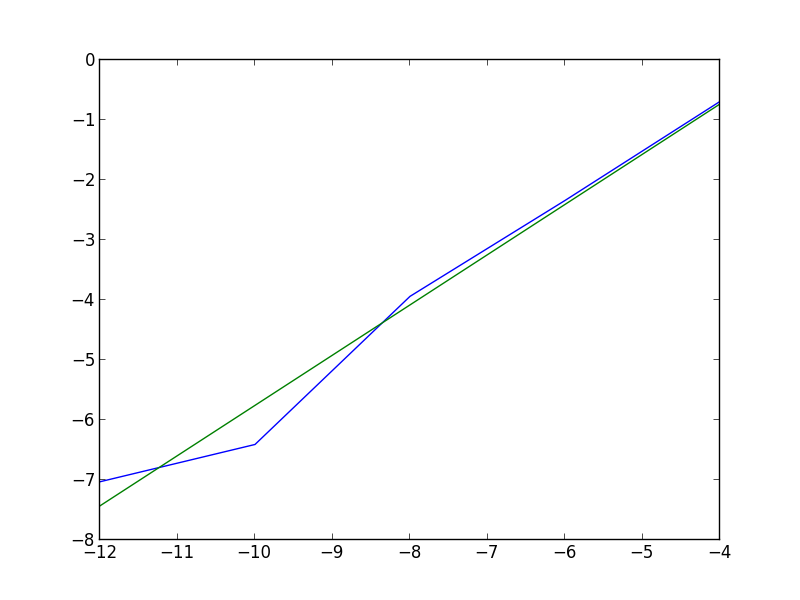
\includegraphics[width=\textwidth,
keepaspectratio]{ex10_em_w.png}
\end{minipage}
\hspace{4mm}
\begin{minipage}[c]{.47\textwidth}
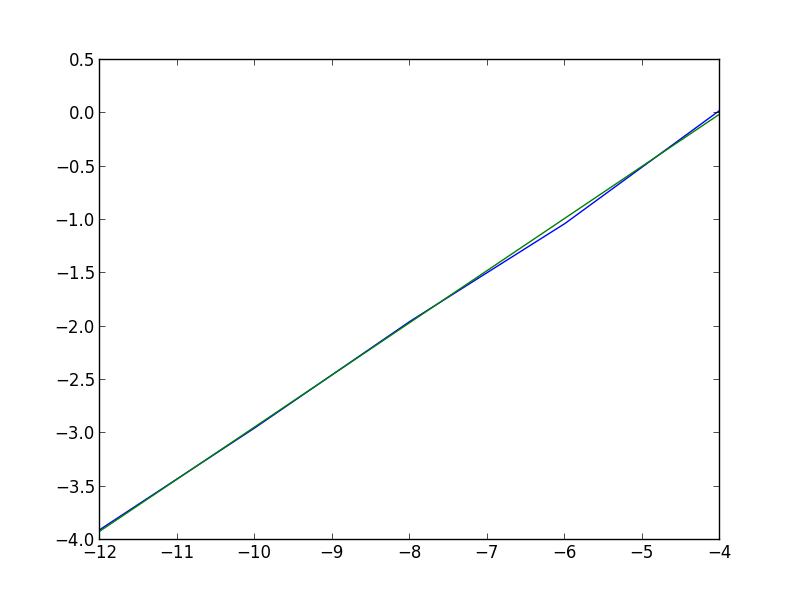
\includegraphics[width=\textwidth,
keepaspectratio]{ex10_em_s.png}
\end{minipage}
\caption{ \label{figure:ex10_em} Weak (left) and strong (right) convergence of the Euler-Maruyama method for equation (\ref{eq:conv_num}).}
\end{figure}
The empirical values of $\alpha$ (i.e. the order of convergence) are $\alpha = 0.84$ and $\alpha = 0.48$ for weak and strong convergence respectively.

\paragraph*{(b)}

We implemented the Milstein scheme for the SDE (\ref{eq:conv_num}).
In Figure (\ref{figure:ex10_mil}), we plot (in logarithmic scale) the error for weak and strong convergence for $T=1$ and $\Delta t = 4^{-i}$, $i=2,\dots,6$, vs the best-fit line.
\begin{figure}[htbp]
\centering
\begin{minipage}[c]{.47\textwidth}
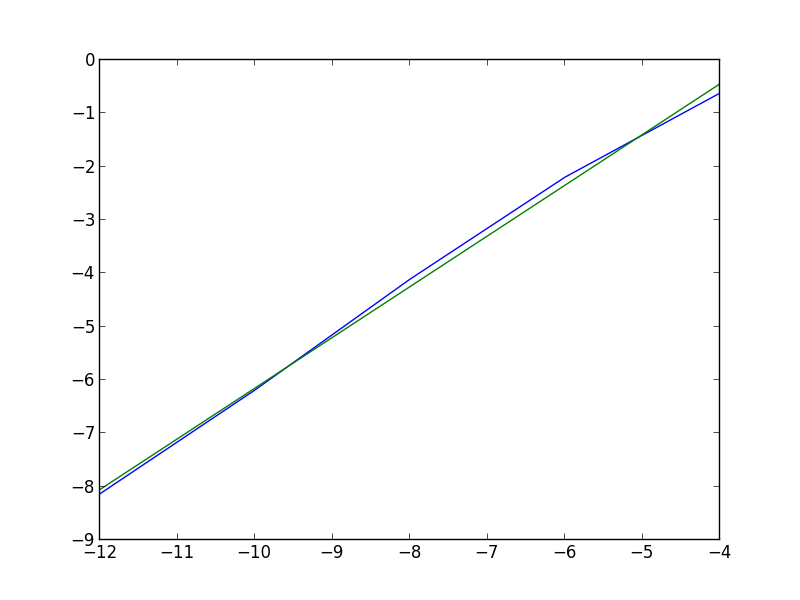
\includegraphics[width=\textwidth,
keepaspectratio]{ex10_mil_w.png}
\end{minipage}
\hspace{4mm}
\begin{minipage}[c]{.47\textwidth}
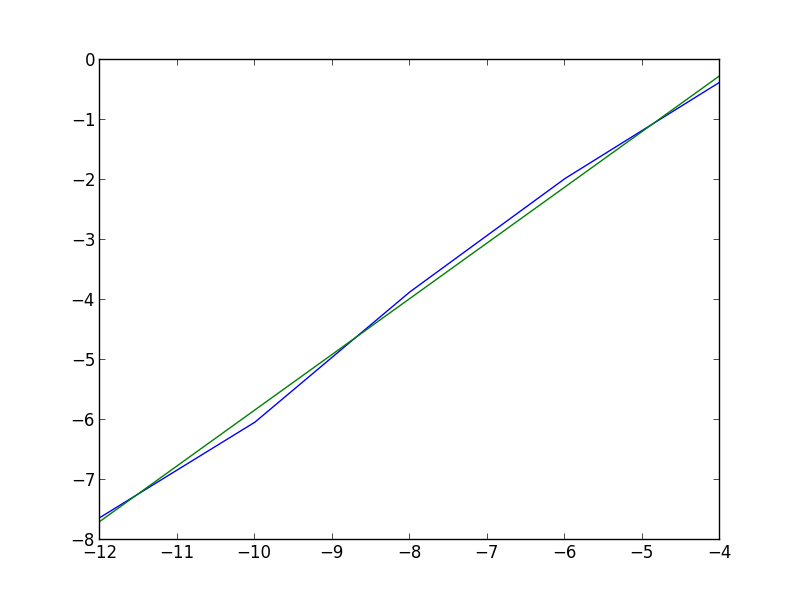
\includegraphics[width=\textwidth,
keepaspectratio]{ex10_mil_s.png}
\end{minipage}
\caption{ \label{figure:ex10_mil} Weak (left) and strong (right) convergence of the Euler-Maruyama method for equation (\ref{eq:conv_num}).}
\end{figure}
The empirical values of $\alpha$ (i.e. the order of convergence) are $\alpha = 0.95$ and $\alpha = 0.92$ for weak and strong convergence respectively.

\paragraph*{(c)}

We implemented the Milstein scheme for the SDE:
\begin{equation}\label{eq:mean_square}
dX_t = -3X_t\,dt + \sqrt{3}X_t\,dW_t, \qquad X_0 = 1
\end{equation}
and we approximated $\lim_{t\to\infty}\expval X_t^2\simeq\expval X_{10}^2$. We found that for $\Delta_1 t = 0.4$ the scheme is unstable ($\expval X_{10}^2\simeq70902$) while for $\Delta_0 t = 0.2$ the scheme is stable ($\expval X_{10}^2\simeq1.012\cdot10^{-20}$).

\paragraph*{(d)}

We implemented the Milstein scheme for the SDE:
\begin{equation}\label{eq:prob}
dX_t = -\frac{1}{2}X_t\,dt + \sqrt{6}X_t\,dW_t, \qquad X_0 = 1.
\end{equation}
and we approximated $P\bra*{\lim_{t\to\infty}\expval \abs{X_t}=0}\simeq P\bra*{\abs{X_{10}}>10^{-5}}$. We found that for $\Delta_1 t = 0.4$ the scheme is unstable ($ P\bra*{\abs{X_{10}}>10^{-5}}\simeq0.722$) while for $\Delta_0 t = 0.2$ the scheme is stable ($P\bra*{\abs{X_{10}}>10^{-5}}\simeq0.999$).

\end{document}